% --------------------------------------------------------------------------%
% Report template for ITV projects
% --------------------------------------------------------------------------%
% Report template with support for Portuguese and English languages
% Change language {brazil or english} in \documentclass as per the examples
% This template has support for the ABNT citing format
% 
% This report template was 
% created by Hector Azpurua (hector.azpurua@itv.org)
% Original version: dec/2017
% https://github.com/h3ct0r/itv_report_latex_template/
% 
% Based on ABNTEX2 and the thesis template
% by Gabriel Garcia (gabrcg@gmail.com)
% --------------------------------------------------------------------------% 

% ------------------------------- %
% Definição de IDIOMA do template %
% ------------------------------- %
\documentclass[
% -- opções da classe memoir --
12pt,					% tamanho da fonte
openright,				% capítulos começam em pág ímpar (insere página vazia caso preciso)
oneside,				% para impressão em verso e anverso. Oposto a oneside
a4paper,				% tamanho do papel. 
% -- opções da classe abntex2 --
chapter=TITLE,			% títulos de capítulos convertidos em letras maiúsculas
%section=TITLE,			% títulos de seções convertidos em letras maiúsculas
%subsection=TITLE,		% títulos de subseções convertidos em letras maiúsculas
%subsubsection=TITLE,	% títulos de subsubseções convertidos em letras maiúsculas
%
% -------------------------------------------------------------- %
% --             Opções de IDIOMA do pacote babel             --
%
% O último idioma é o principal do documento
% *NÃO* deixar espaços/newlines embaixo do ultimo idioma
%
% -- Descomentar para idioma inglês
%brazil,
%english
%
% Descomentar para idioma Português
english,
brazil
% -------------------------------------------------------------- %
]{abnt/abntex2itv_report}

\usepackage[utf8]{inputenc}		% Codificacao do documento (conversão automática dos acentos)
\usepackage{lastpage}			% Usado pela Ficha catalográfica
\usepackage{indentfirst}		% Indenta o primeiro parágrafo de cada seção.
\usepackage[table,xcdraw]{xcolor}				% Controle das cores
\usepackage{graphicx}			
\usepackage{microtype} 			% para melhorias de justificação
\usepackage{supertabular}       % tabela na capa do documento
\usepackage{booktabs}
\usepackage{adjustbox}
\usepackage{amssymb,amsmath,mathrsfs}
\usepackage{algorithm,algpseudocode}
\usepackage{pgfplots}
\usepackage{tikz}
\usepackage{lipsum}	
\hypersetup{draft}
\usepackage{ragged2e}
\usepackage{tocloft}
\usepackage{etoolbox}
\usepackage[brazilian,hyperpageref]{backref} % Paginas com as citações na bibliografia
\usepackage[alf,abnt-etal-list=0,abnt-etal-cite=3,abnt-emphasize=bf]{abntex2cite}
\usepackage[normalem]{ulem}
\usepackage{yaacro}
%\usepackage{lscape}
%\usepackage{rotating}

%other packages
\usepackage[T1]{fontenc}
\usepackage{lmodern}

\usepackage[none]{verlab}

% -------------------------- %
% Configurações do PDF final %
% -------------------------- %
\definecolor{blue}{RGB}{41,5,195}
\makeatletter
\hypersetup{
	%pagebackref=true,
	pdftitle={\@title}, 
	pdfauthor={\@author},
	pdfsubject={\@title},
	pdfcreator={LaTeX with abnTeX2},
	pdfkeywords={abnt}{latex}{abntex}{abntex2}{\imprimirpalavraschave}, 
	colorlinks=true,       		% false: boxed links; true: colored links
	linkcolor=blue,          	% color of internal links
	citecolor=blue,        		% color of links to bibliography
	filecolor=magenta,      	% color of file links
	urlcolor=blue,
	bookmarksdepth=4
}
\makeatother

% ---------- %
% Formatação %
% ---------- %
\apptocmd{\thebibliography}{\justifying}{}{} 
\renewcommand{\ABNTEXsectionfont}{\bfseries}
\setlength{\cftsectionindent}{0em}
\setlength{\cftsubsectionindent}{0em}
\setlength{\cftsubsubsectionindent}{0em}

\AtBeginDocument{
	\addtocontents{toc}{\normalsize}
}

% \makeatletter
% \newcommand{\todo}[1]{{\color{red}\textbf{{\large @TODO\@ifempty{#1}{}{: }}#1}}}
% \newcommand{\reviewtext}[1]{{\color{blue}#1}}
% \makeatother

% Rearranja os finais de cada estrutura
\algrenewtext{EndWhile}{\algorithmicend\ \algorithmicwhile}
\algrenewtext{EndFor}{\algorithmicend\ \algorithmicfor}
\algrenewtext{EndIf}{\algorithmicend\ \algorithmicif}
\algrenewtext{EndFunction}{\algorithmicend\ \algorithmicfunction}

% Espaçamentos entre linhas e parágrafos 
% O tamanho do parágrafo é dado por:
\setlength{\parindent}{1.3cm}
% Controle do espaçamento entre um parágrafo e outro:
\setlength{\parskip}{0.2cm} % tente também \onelineskip

% ------------------------------------------------%
% Informações de dados para CAPA e FOLHA DE ROSTO %
% ------------------------------------------------%
% Explicação e exemplos dos comandos de configuração do template:
% \renewcommand{\ITVlocation}{MI}
% 		Localização do ITV (DS ou MI).
%
% \prodtecnica
%		Número de produção técnica ITV.
%
% \titulo
%		Titulo do relatorio Ex: "Relatorio do estado da arte".
%
% \nomeprojeto
%		Nome do projeto.
%
% \outrossubtitulos
%		Outros subtitulos, pode ser deixado em branco.
%
% \autores
%		Os autores relacionados ao ITV, separados por newline "\\" Ex: Autor 1\\Autor 2\\Autor 3.
%
% \newcommand{\autoresexternos}
%		Os parceiros que participaram no documento, separados por newline pode ser opcional comentando a função.
%
% \local
%		Lugar onde foi realizado o documento. Se for MI o local deve ser "Ouro Preto\\Minas Gerais, Brasil".
%
% \data
%		Data do documento em formato Mês/Ano.
%
% \parceirologo 
%		Logo do parceiro a ser colocado na portada do documento, pode ser opcional comentando a função.

\renewcommand{\ITVlocation}{MI}
\prodtecnica{N001/2077\\DOI:00.00000/PROD.TEC.ITV.Snow}
\titulo{Report Title/Título do relatorio}
\nomeprojeto{Project name/Nome do projeto}
\outrossubtitulos{~} % opcional

\autores{
	\small
	Jon Snow\\
	Son Goku\\
	Megaman X7 Maverick\\
	Conan The Barbarian
}

\newcommand{\autoresexternos}{ % optional
	Cleyton Dias\\
	Gabriel Garcia\\
	Jhonson Santos\\
	Robson Gomes
}

\local{Ouro Preto\\Minas Gerais, Brasil}
\data{Março/2020}
\parceirologo{logos/logo_parceiro_base.png} % optional

% --------------------------------------%
% Finalização das configurações da capa %
% --------------------------------------%

% ----------------------------- %
% Acronimos                     %
% ----------------------------- %
% Chamar no texto como \ac{DoF} %
% ----------------------------- %
\begin{acgroupdef}[list=acronyms]
	\acdef{DoF}{Degrees of Freedom}
	\acdef{FRVF}{Forbidden Region Virtual Fixture}
	\acdef{GVF}{Guidance Virtual Fixture}
	\acdef{LHD}{Load-Haul-Dump}
	\acdef{SLAM}{Simultaneous Localization and Mapping}
\end{acgroupdef}

\makeindex

\begin{document}
	
	\frenchspacing
	
	\imprimircapa
	
	% ------------------- %
	% Ficha Catalográfica %
	% ------------------- %
	{
		% Usar a ficha catalográfica gerada pela biblioteca do ITV em formato PDF
		\begin{figure}[H]
			\centering
			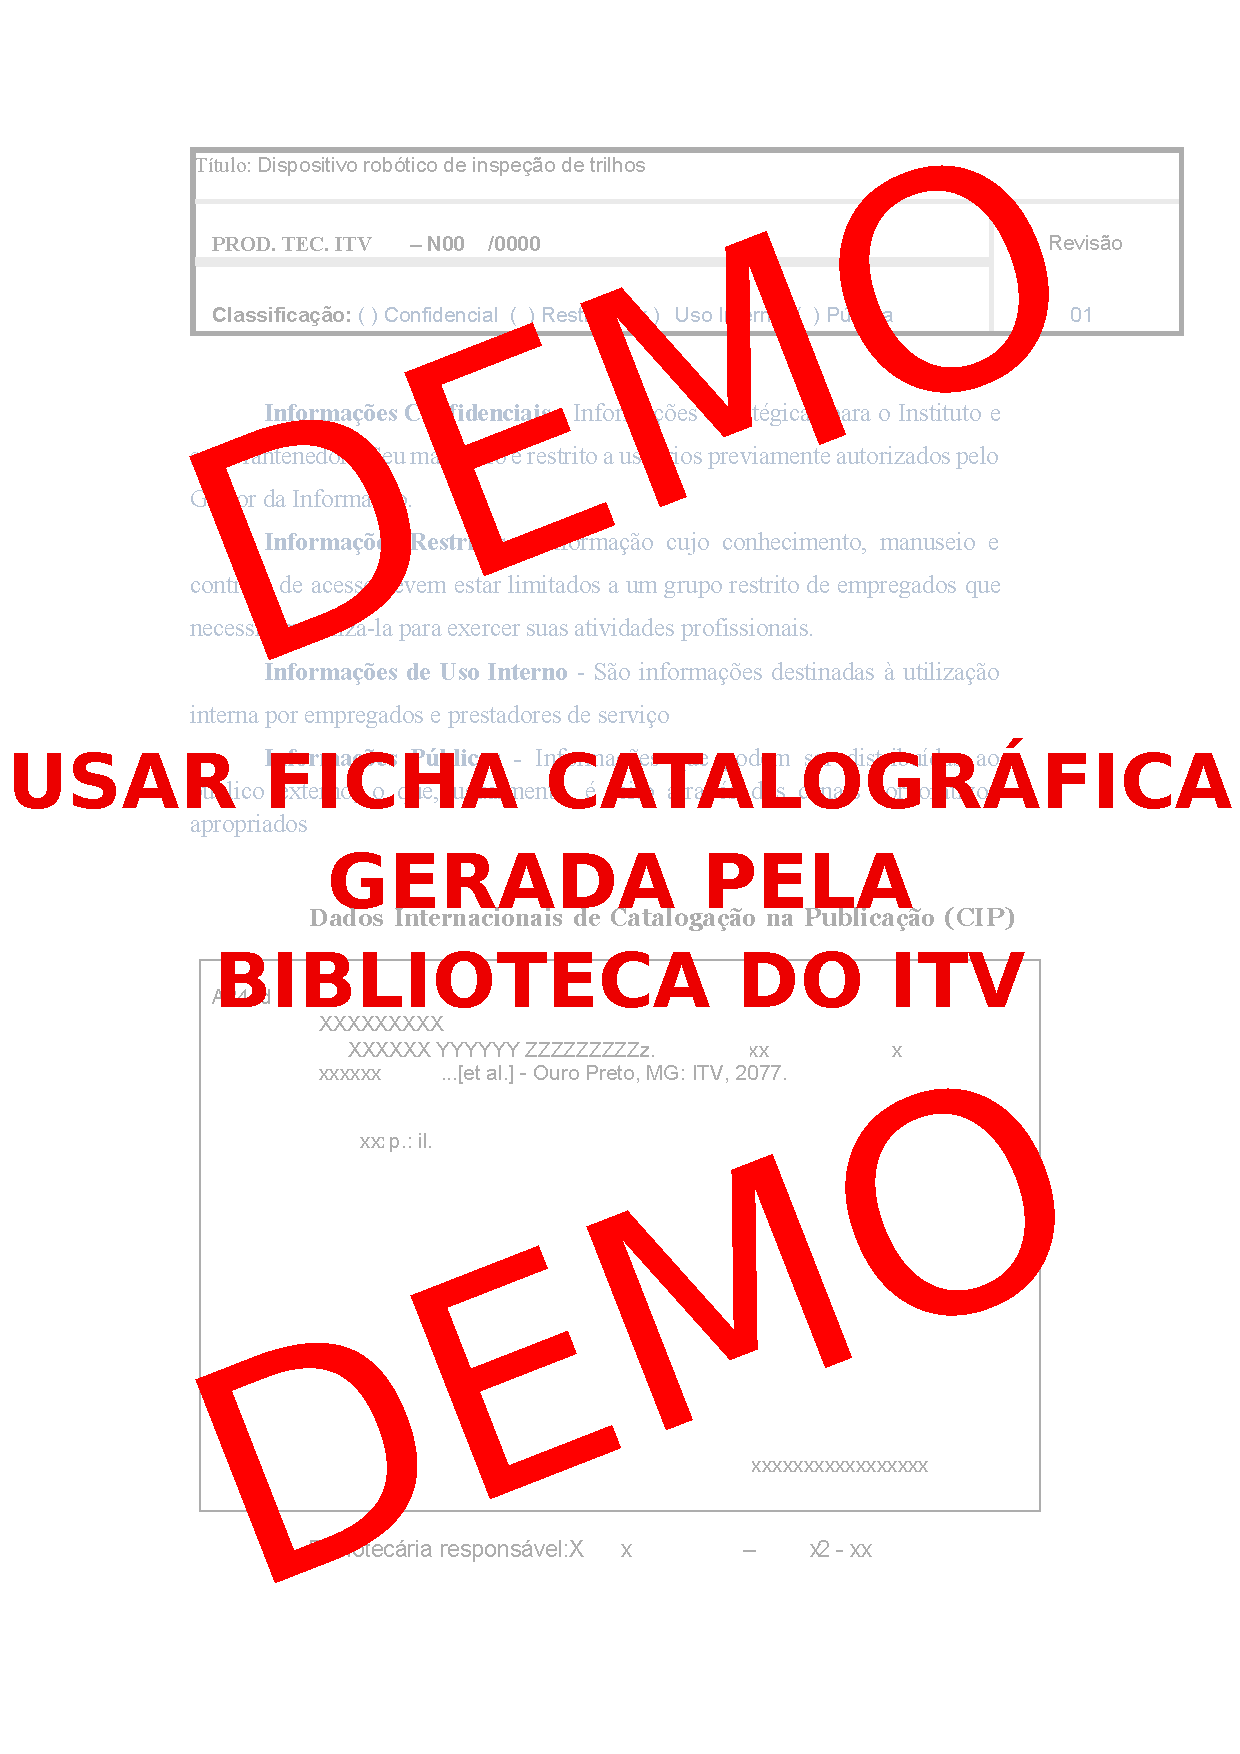
\includegraphics[width=0.99\linewidth]{img/examples/ficha_catalografica_demo.pdf} %usar linewidth ao invés de textwidth
		\end{figure}
		
		\cleardoublepage
	}
	
	% ---------------- %
	% Resumo executivo %
	% ---------------- %
	\centering
	\ABNTEXchapterfont\large\textbf{\execsummarytitlename}
	\begin{flushleft}
		\normalsize
		\justify
		\normalfont
		
		\lipsum[2] % Comentar e adicionar resumo executivo aqui
	\end{flushleft}
	\clearpage
	
	% ----------------- %
	% Resumo e abstract %
	% ----------------- %
	\ABNTEXchapterfont\large\textbf{\resumoatitlename}
	\begin{flushleft}
		\normalsize
		\justify
		\normalfont
		
		\lipsum[2] % Comentar e adicionar resumo aqui
		\noindent\textbf{Palavras-chave:} Keyword 1. Keyword 2. Keyword 3. Keyword 4.
	\end{flushleft}
	
	\vspace*{1cm}
	
	\ABNTEXchapterfont\large\textbf{\resumobtitlename}
	\begin{flushleft}
		\normalsize
		\justify
		\normalfont
		
		\lipsum[2] % Comentar e adicionar resumo em ingles aqui
		
		\noindent\textbf{Keywords:} Keyword 1. Keyword 2. Keyword 3. Keyword 4.
	\end{flushleft}
	\clearpage
	
	
	% ---------------- %
	% Lista de figuras %
	% ---------------- %
	\ABNTEXchapterfont\Large\textbf{\MakeUppercase\listadefigurasname}
	\vspace*{-24pt}
	\pdfbookmark[0]{\listfigurename}{lof}
	\normalsize
	\listoffigures*
	\cleardoublepage
	
	
	% ---------------- %
	% Lista de tabelas %
	% ---------------- %
	\ABNTEXchapterfont\Large\textbf{\MakeUppercase\listadetabelasname}
	\vspace*{-24pt}
	\pdfbookmark[0]{\listtablename}{lot}
	\normalsize
	\listoftables*
	\cleardoublepage
	
	
	% -------------------------- %
	% Lista de simbolos e abrev. %
	% -------------------------- %
	\begin{centering}
		\ABNTEXchapterfont\Large\textbf{\MakeUppercase\listadesimbolsabrevtitlename}
		\noindent
		\normalsize
		\normalfont
		\aclist[list=acronyms]
	\end{centering}
	\newpage
	
	% 	\newpage
	% ------------------ %
	% Tabela de conteudo %
	% ------------------ %
	\ABNTEXchapterfont\Large\textbf{\MakeUppercase\glosariotitlename}
	\vspace*{-24pt}
	\pdfbookmark[0]{\contentsname}{toc}
	\normalsize
	\normalfont
	\tableofcontents*
	\justify
	\cleardoublepage
	
	% ------------------------------ %
	% Conteudo do relatorio **AQUI** %
	% ------------------------------ %
	% Formatação, remover espaço depois dos titulos
	\setlength\beforechapskip{-24pt}
	\setlength\afterchapskip{12pt}
	\textual
	\pagestyle{plain}
	\normalsize
	%\justify
	\normalfont
	
	\input{\ITVexemplotex} % Exemplo de uso
	% use \include to include different chapters
	% for example:
	% \input{sections/1_introduction}
	
	% ----------- %
	% Referências %
	% ----------- %
	\cleardoublepage
%	\titleformat{\chapter}[display]{\vspace*{-24pt}\ABNTEXchapterfont\centering\large\bfseries}{\chaptertitlename\ \thechapter}{12pt}{\Large}
%	
%	\ABNTEXchapterfont\centering\Large\textbf{\MakeUppercase{\anexosname}}
	\bibliography{bibliography}
	
	% -------- %
	% Apêndice %
	% -------- %
	% 	\apendices
	% 	\justify
	% 	\chapter{\ITVtitlename}
	
	% 	\lipsum[1] % Comentar e adicionar apêndice aqui
	
	% ----- %
	% Anexo %
	% ----- %
	\newpage
	\begin{flushleft}
		\ABNTEXchapterfont\centering\Large\textbf{\MakeUppercase{\anexosname}}
	\end{flushleft}
	\vspace*{-36pt}
	\pdfbookmark[0]{\contentsname}{toc}
	\normalsize
	\normalfont
	\justify
	
	\anexos
	\justify
	\centering
	\chapter{XXXXX}
	\label{chapter:anexo1}
	
	\lipsum[1].
	
	\begin{figure}[htbp] %NÃO usar H, usar htbp
		\centering
		\caption{Lorem ipsum dolor sit amet, consectetur adipiscing elit. Sed aliquam, arcu vel rutrum fermentum, ex sem tempus odio, eget congue dolor lacus et justo.}
		\label{fig:annex1}
		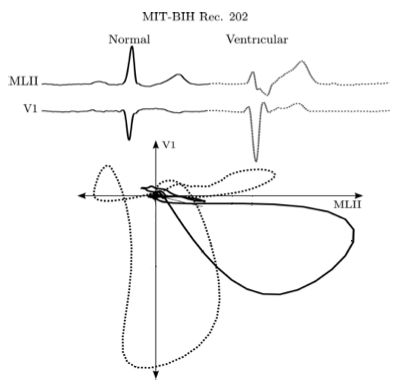
\includegraphics[width=0.65\linewidth]{img/examples/vcg.png} %usar linewidth ao invés de textwidth
		\legend{Fonte: Os autores.}
	\end{figure}
	
\end{document}